

\documentclass[oneside,a4paper,12pt]{article}
\usepackage{graphicx}
\usepackage{amsmath}
\usepackage{listings}
\lstset{language=html}
\usepackage{array}
\usepackage{biblatex}
\addbibresource{rapport.bib}
\usepackage{hyperref}
\graphicspath{{~/templates/}, {../images/}}

\makeindex
\begin{document}
	\begin{titlepage}
		\includegraphics[width=4cm]{logopopo.png}
		\hspace*{\fill}
		\includegraphics[width=6cm]{logouniv.png}
		
		\begin{center}
			\vspace{1cm}
			\textbf{Mémoire de Stage de 4e année}\\
			\vspace{1cm}
			\textbf{\LARGE FL-Minifer}\\
			\textbf{\large A Tool To Minify and Unify AdBlocker’s Filter Lists}\\
			\vspace{1cm}
			\textbf{Maxence NEUS}\\
			\vspace{1cm}
			\begin{tabular}{ c c }
				
\includegraphics[width=6cm]{logoInria.jpg} & 
\includegraphics[width=6cm]{logospirals.png}\\
			\end{tabular}

			\vspace{2cm}

			\begin{tabular}{ m{6cm} | m{6cm} }
				\textbf{Polytech Lille} & \textbf{Inria} \\
				\hline
				& \\
				Secrétariat - Bureau & 40 Av. Halley \\
				Boulevard Paul Langevin - Cité Scientifique & 59650 Villeneuve d'Ascq \\
				59655 VILLENEUVE D’ASCQ CEDEX & Tuteur Entreprise : \\
				03-28-76-73-60 & \textbf{Walter RUDAMETKIN} \\
				03-28-76-73-61 & Tuteur Ecole \\
				\includegraphics[width=2.5cm]{logouniv.png} \includegraphics[width=2.5cm]{logopopo.png} & \textbf{Walter RUDAMETKIN} \\
				
			\end{tabular}
			
			\vspace{\fill}
			\textbf{2022}\\
		\end{center}
	\end{titlepage}

\tableofcontents

\newpage

\begin{figure}[h]
	\centering
	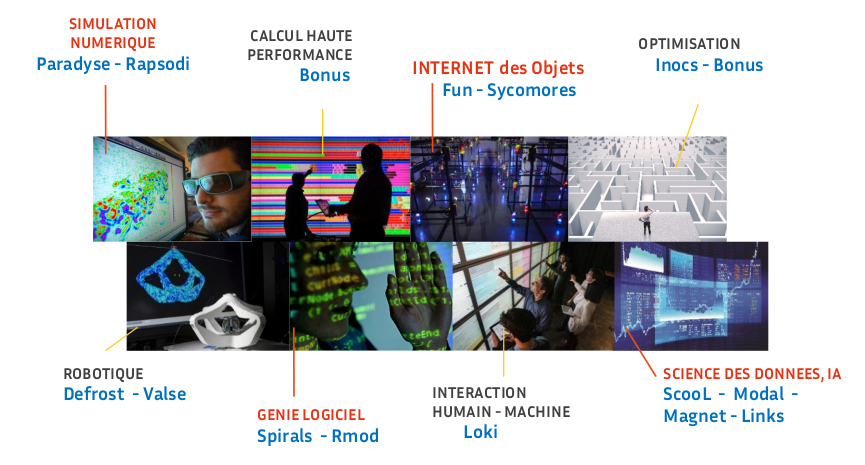
\includegraphics[width=0.55\textwidth]{equipesCentre.png}
	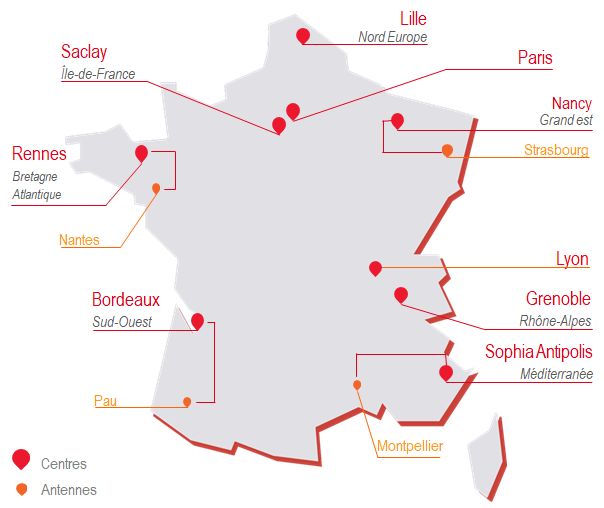
\includegraphics[width=0.4\textwidth]{cartecentres.png}
\end{figure}

\section{Présentation de l'entreprise}
\subsection{Inria}
Inria est l’institut national de recherche en sciences et technologies du numérique. La recherche de rang mondial, l’innovation technologique et le risque entrepreneurial constituent son ADN. Au sein de 200 équipes-projets, pour la plupart communes avec les grandes universités de recherche, plus de 3 900 chercheurs et ingénieurs y explorent des voies nouvelles, souvent dans l’interdisciplinarité et en collaboration avec des partenaires industriels pour répondre à des défis ambitieux.
Institut technologique, Inria soutient la diversité des voies de l’innovation : de l’édition open source de logiciels à la création de startups technologiques (Deeptech).

\begin{figure}[h]
	\centering
	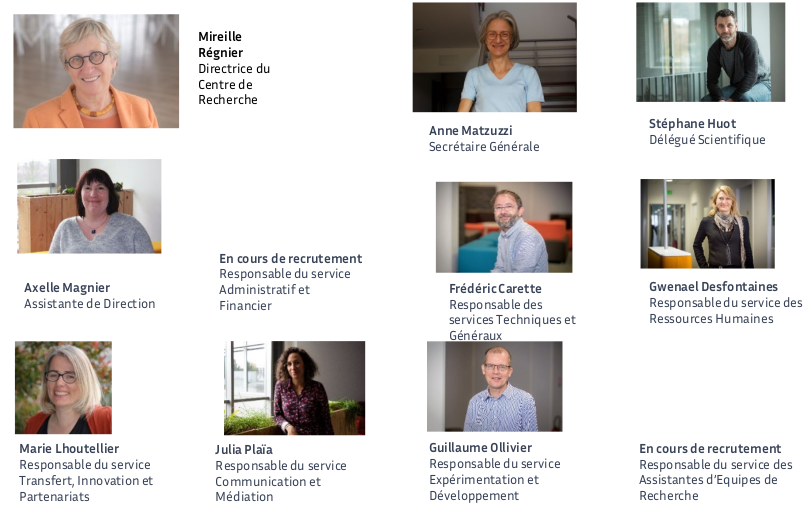
\includegraphics[width=10cm]{direction.png}
	\caption{\'Equipe de direction}
\end{figure}

\subsection{L'équipe Spirals}
L'équipe Self-adaptation for distributed services and large software systems(ou SPIRALS) mène des activités de recherche dans les domaines des systèmes répartis et des sciences du logiciel. 
Elle a pour but d'introduire plus d'autonomie dans les mécanismes d'adaptation des systèmes logiciels, en particulier, afin d'assurer la transition des systèmes adaptatifs vers les systèmes auto-adaptatifs. 
Elle vise plus particulièrement deux propriétés : l'auto-guérison et l'auto-optimisation. 
Avec l'auto-guérison, elle a pour but d'étudier et d'adapter des solutions de fouille de données et d'apprentissage à la conception et la mise en œuvre de systèmes logiciels, plus particulièrement en vue de la réparation automatique des systèmes logiciels. 
Avec l'auto-optimisation, elle a pour but de partager, collecter et analyser les comportements dans un environnement réparti afin de continuellement adapter, optimiser et maintenir en fonctionnement des systèmes logiciels et d'aller vers l'obtention de systèmes distribués éternels.
L'équipe est composée de doctorants, de post-doctorants et d'Ingénieurs. L'équipe est multiculturelle ; la langue majoritairement utilisée pour communiquer dans les réunions et en groupe a donc été d'anglais.


\subsection{Le développement durable dans l'entreprise}
Inria s’engage dans une démarche de développement durable. Les deux axes privilégiés sont l'informatique durable et les déplacements ; l'institut s'est doté d'une "commission nationale développement durable" chargée de définir un plan pluriannuel de travail et de "commissions locales du développement durable" qui devront mettre en œuvre des préconisations en intégrant les contraintes et spécificités de chaque site.

Le bâtiment dans lequel j'ai passé mon stage est caractérisé comme "un bâtiment de basse consommation" : il restreint les consommations et en arrête certaines comme l'électricité la nuit.



\newpage

\section{Contexte du projet}
\subsection{Introduction aux adBlockers}\label{Intro:adblock}

\paragraph*{Les cookies:}

Le modèle économique du web est centré autour des données utilisateur et de la façon dont elles sont utilisées, majoritairement pour cibler au mieux des publicités qui pourront alors faire un maximum de conversions (nombres d'achats par publicité imprimée sur une page). Évidement pour cibler efficacement un utilisateur il est nécessaire de pouvoir associer un ensemble de données à un utilisateur, historiquement les cookies ont été l'outil le plus rependu pour remplir cette fonction: en incorporant un identifiant unique à chaque utilisateur dans ses requêtes HTML.\\

Malheureusement pour les géants du web, l'idée que quelques entreprises puissent avoir accès à une quantité alarmante de leurs données simplement par leur navigation sur le web ne plait pas vraiment aux utilisateurs. Suite à des campagnes de sensibilisation de plus en plus d'utilisateurs du web se sont retrouvés confrontés à cette réalité et désirent autant que possible limiter l'accès à leurs données de navigation. Pour cela plusieurs compagnies se sont misent à créer des extensions pour navigateurs qui permettent de bloquer les dis ``tracking cookies''. En effet tous les cookies n'ont pas pour but de traquer l'utilisateur, la technologie a été créée pour garder des informations utilisateurs essentielles à la fonctionnalité du site comme rester connecter à son compte utilisateur ou sauvegarder l'état du panier sur les sites de shopping en ligne. Ces cookies dits ``essentiels'' doivent être filtrés pour garder les fonctionnalités du site, une méthode largement utilisée est de bloquer les cookies dits ``tierces'' qui proviennent de domaines différents de celui du site visité étant donné que ceux ci sont bien souvent utilisés uniquement comme tracking cookies et peuvent donc être bloqués sans crainte de nuire aux fonctionnalités du site.

\paragraph*{La publicité sur le web:}

Comme dit précédemment, le modèle économique du web consiste à montrer le plus de publicités intéressantes possible à l'utilisateur pour qu'il achète le plus de produits possible. Ce modèle entraîne logiquement un comportement où les sites utilisent chaque pixel d'espace libre de contenu sur leurs sites pour y servir des publicités grâce à un modèle d'enchères où les distributeurs de publicités enchérissent le plus sur les utilisateurs avec un intérêt probable pour leurs produits.

Les utilisateurs veulent donc se débarrasser un maximum des publicités à la fois pour leur confort mais aussi pour protéger les plus vulnérables des pratiques prédatoriales des entreprises. C'est là l'utilité des adBlockers qui scannent les éléments de la page et bloquent ceux qui sont détectés comme étant des publicités.

\paragraph{Les rêgles de filtrage:}\label{Intro:adblock:filterlists}

Pour détecter les éléments qui font parties de publicités, les adBlockers utilisent des listes de filtres qui contiennent des caractéristiques d'élements publicitaires rencontrés sur le web. Ces listes sont maintenus régulièrement par la communauté et par des entreprises d'adBlockers pour parer aux nouvelles tentatives de contournement des distributeurs de publicités. Les listes sont de simples fichiers texte dont la syntaxe de base est définie par AdBlockPlus (ABP) \href{https://help.eyeo.com/en/adblockplus/how-to-write-filters#allowlist}{ici} et elle est étendue par uBlockOrigin (uBO) \href{https://github.com/gorhill/uBlock/wiki/Static-filter-syntax#extended-syntax}{ici}. La syntaxe comporte deux grands types de règles: 
\begin{itemize}
\item Les \textit{Network Rules}
\item Les \textit{Cosmetic Rules}
\end{itemize}
Le cas le plus simple, les \textit{Network Rules} correspondent à des rêgles qui bloquent les éléments selon l'url dont ils sont importés, ce grâce à une syntaxe similaire à des expressions régulières. C'est à dire que la règle décrits un modèle d'url qui correspond à un ensemble d'url qui devront être bloquées, par exemple ``http://example.com/ads/banner*.gif'' bloquera les éléments venant de la source ``http://example.com/ads/banner420.gif'' (le caractère \textbf{*}\\ correspondant à n'importe quelle suite de caractère) mais pas \\``http://example.fr/ads/ad123.png''.

Plus puissantes, les \textit{Cosmetic Rules} bloquent des éléments dont le css correspond à une certaine description, par exemple la règle ``\#\#\#ad-boxes'' bloque les éléments sur la page qui ont une id css de ``ad-boxes''.

Il est également possible d'écrire des exceptions qui permettent de laisser passer des élements qui seraient bloqués par une règle trop générale et qui nuirait aux fonctionnalités du site.

\subsection{Présentation AmIUnique}\label{Intro:amiunique}

\paragraph*{Le Fingerprinting sur le web}

Comme décrit en \ref{Intro:adblock} les cookies ont longtemps été l'outil principal pour suivre les utilisateurs sur le web, mais les efforts des adBlockers et des navigateurs comme Firefox ou Brave ont rendus leurs utilisation plus difficile ou moins efficaces qu'avant, et avec la demande pour les données utilisateur encore grimpante, de nouveaux outils plus avancés sont développés pour continuer à suivre les utilisateurs sur le web. 

Un outil qui remplis cette fonction peut-être mieux encore que les cookies le faisaient auparavant est le \textbf{Browser Fingerprinting} (\cite{fingerprinting}) le principe derrière celui-ci consiste à appliquer une approche inspirée de la \textit{data science} et d'obtenir un maximum de bribes d'information sur l'utilisateur (ou ici plutôt son navigateur) afin de les agréger en un identificateur unique permettant de suivre l'utilisateur grâce à la configuration de son navigateur que les cookies soit acceptés ou non.

\paragraph*{AmIUnique} est un projet d'Inria Lille qui consiste à étudier les caractéristiques du navigateur qui permettent de l'identifier et de faire des statistiques sur les changements de l'identificateur au cours du temps grâce à une extension qui collecte les informations d'identification. Le site \href{https://www.amiunique.org}{amiunique.org} comporte une partie où l'utilisateur peut visualiser les caractéristiques de sa configuration qui peuvent permettre de l'identifier avec une indication de la quantité d'information obtenue pour chaque item par un ``Taux d'unicité'' qui donne la proportion des configurations relevées qui partagent chaque item de configuration avec vous.\\

Le site comporte également une page qui permet de découvrir quelles listes de filtre (\ref{Intro:adblock:filterlists}) sont installées sur le navigateur, le but étant d'illustrer un potentiel nouveau point de données qui pourrait être ajouté au fingerprint du navigateur. L'expérience est poussée un cran plus loin avec une page qui tente de déterminer les versions spécifiques des listes installées pour obtenir plus de données susceptibles d'identifier l'utilisateur.

Pour réaliser cette fonctionnalité, l'application a besoin de trois choses :
\begin{itemize}
	\item Un ensemble de listes de filtres à tester avec un maximum de versions possibles
	\item Une façon de tester les règles pour voir si elles sont présentes sur le système
	\item Un algorithme capable à partir de l'ensemble des règles bloquées de déterminer si une liste est présente ou non
\end{itemize}

La première partie est réalisée par une application basée sur l'outil \textit{Airflow}, développé par Apache, qui permet de gérer une chaine de procédures (ici des notebooks jupyter) et de s'assurer du bon fonctionnement de la pipeline grâce à un monitoring notebook par notebook et avec la possibilité d'alerter par mail d'erreurs lors de l'execution.

Le but de la pipeline \textit{Airflow} est de récupérer les dernières versions des listes de filtres (à interval régulier) afin d'effectuer un premier traitement sur celles-ci qui préparera le travail pour la partie algorithmique de détection de liste. Ce pré-processing consiste à créer une couverture par ensembles (cf. annexe \ref{setcover}) où l'univers est l'ensemble des règles contenues dans toutes les listes considérées. Le but de cette approche est de trouver un ensemble de parties de l'univers comme suit:

Pour tester si les règles sont présentes ou non sur le navigateur, la page de test insère des éléments html qui correspondent à des \textit{Network Rules} faisant partie de l'ensemble déterminé précédemment, ces éléments sont de la forme:]
\begin{center}
\begin{lstlisting}
   <img src='source' style='visibility: hidden' />
\end{lstlisting}
\end{center}

On peut alors vérifier une fois la page chargée pour chaque élément si il est visible ou non et alors utiliser l'algorithme associé à la couverture par ensembles déterminées précédemment pour déterminer quelles listes sont installées sur le navigateur.\\

On peut utiliser le même raisonnement lors de la détection des versions en traitant simplement chaque version différente de la liste comme étant une liste différente.


\section{Corps du projet}\label{Projet}

Le but global du stage est d'étendre et d'améliorer AmIUnique, plus particulièrement la partie qui concerne les listes de filtres. En effet un des buts de l'étude est d'observer les résultats du fingerprinting et ses changements au cours du temps pour un utilisateur donné afin de mesurer la faisabilité d'un suivi longue durée d'un utilisateur à travers le web.
Or avec simplement une page web, on aurait besoin que les utilisateurs passe régulièrement sur le site pour vérifier leur fingerprint, ce qui est peu probable pour un grand nombre d'utilisateurs.
C'est le rôle de l'extension, mais elle ne comporte actuellement pas la détection de listes de filtres. La création d'une extension qui inclue ces fonctionnalités fait partie de mes missions lors de ce stage. D'autres améliorations pour l'extension telles que des visualisations des changements de fingerprint au cours du temps seront également explorées.

\subsection{Extension Chrome}\label{Projet:extension}

Dans un premier temps il m'a fallu comprendre le fonctionnement global d'une extension chrome. Ces extensions sont programmée en \textbf{javascript} et utilisent l'API chrome.extension qui implémente un nombre d'évenements et de méthodes permettant d'intéragir avec les fenêtres et les onglets. 

Pour notre application, on peut adopter une architecture composée d'un \textit{Background script} qui communique avec des \textit{Content script} via des messages. 
\paragraph*{Le \textit{Background script}} contient du code qui tourne tout au long de la session (c'est à dire depuis l'ouverture d'une fenêtre jusqu'à sa fermeture) et il a pour but principal de gérer la communication avec les différents \textit{Content script} et de gérer l'ensemble des données nécessaires au fonctionnement de l'extension.
\paragraph*{Les \textit{Content scripts}} eux, sont instanciés par le \textit{Background script} ou par un événement extérieur (dans notre cas il sera instancié par l'évenement \lstinline{``document-start''} qui est lancé à chaque fois qu'une page commence à charger).\\

Notre extension a pour but d'émuler le comportement de la page de test mais sans avoir besoin que l'utilisateur ne change ses habitudes de navigation. Pour réaliser cette fonction on propose le processus suivant:\\

\`A chaque chargement de page l'extension insère les mêmes éléments de tests que le site web via un \textit{Constent script} et renvoie les résultats au \textit{Background script} où les résultats sont analysées par l'algorithme de couverture par ensembles de la même manière qu'avec le site web.\\

Pour les \textit{Network rules}, cette démarche fonctionne sensiblement identiquement à la page de test. Cependant pour ce qui est des \textit{Cosmetic rules}, il apparait des contraintes plutôt surprenantes. En effet sur certains sites aucun des éléments insérés ne sont bloqués malgré qu'il existe une rêgle installée qui devrait s'appliquer. Suite à de nombreux tests nous avons déterminer que cela viens de quelques rêgles d'exception qui désactive le bloquage sur les éléments qui viennent de certains domaines (par exemple \lstinline{@@||www.google.*/search?$generichide} qui fait partie de Easylist). Ces domaines correspondent avec les sites sur lesquelles nos éléments ne sont pas bloqués. Cela vient de notre démarche qui utilise les \textit{Content scripts} pour insérer les éléments dans la page, en effet cela fait que la source de l'élément inséré est le script qui tourne sur la page et donc la source correspond à l'url de la page. Ce qui enclanche la rêgle d'exception et nos éléments ne sont pas bloqués. Ce problème apparait aussi lorsque le site visité fait partie des \textit{Trusted sites} sur lequel l'adBlocker est complètement désactivé.\\

Pour pallier à ce problème, la solution proposée est de vérifier après le test si aucun élément n'a été bloqué, si c'est le cas c'est qu'il existe une rêgle d'exception installée pour le site visité ou que le site fait partie de la liste des \textit{Trusted sites} et la batterie de tests est donc ignorée.

\subsection{Optimisations du processus}\label{Projet:opti}

Le second plan du projet de stage consiste à apporter des optimisations et des améliorations à la page de test. En effet celle-ci ne comporte actuellement que des tests sur les \textit{Network rules} et laisse donc un grand nombre de rêgles (\textit{Cosmetic rules}) de côté. Inclure ces \textit{Cosmetic rules} permettrait d'améliorer la précision du modèle, en effet pour les adBlockers, les \textit{Network rules} sont assez limités pour bloquer les publicités plus avancées qui ne servent pas toujours depuis le même domaine. Cela fait que les \textit{Cosmetic rules} forment un grand nombre des rêgles présentes dans les listes et leur omission influe grandement sur le précision du modèle, nottament sur les tests de versions car les \textit{Network rules} varient peu de version en version ce qui rend certaines listes impossibles à tester pour les versions.\\

Par ailleur des optimisations sur l'algorithme de test sont à rechercher également pour améliorer la vitesse d'execution du test et limiter l'utilisation de ressources pour l'extension.\\

\`A l'écriture de ce rapport, ces tâches n'ont pas encore pu être effectuées.

\section{Extras}

\subsection{Organisation}

La proximité avec mes cammarades stagiaires a facilité les échanges et l'entraide notamment au début des projets pour la mise en place des outils de développement et de communication avec le reste de l'équipe.\\

Au sein de l'équipe et d'Inria en général le mode de communication privilégié est \textbf{Mattermost}, un service open source de messagerie instantanée hebergé sur les serveurs d'Inria. Nous avons également accès aux services de mail (\textbf{Zimbra}) et au gitlab de l'Inria.

Pour ce qui est des outils de développement, on utilise nos machines persos pour la majorité des tâches qui ne nécessitent pas de grandes puissances de calculs et on a obtenu l'accès au serveur de développement de \textbf{Spirals} pour réaliser des expériences plus demandantes en ressources.

\subsection{Vie au centre}

\newpage

\appendix

\section{Couvertures par ensembles}\label{setcover}

\begin{figure}[h]
	\centering
	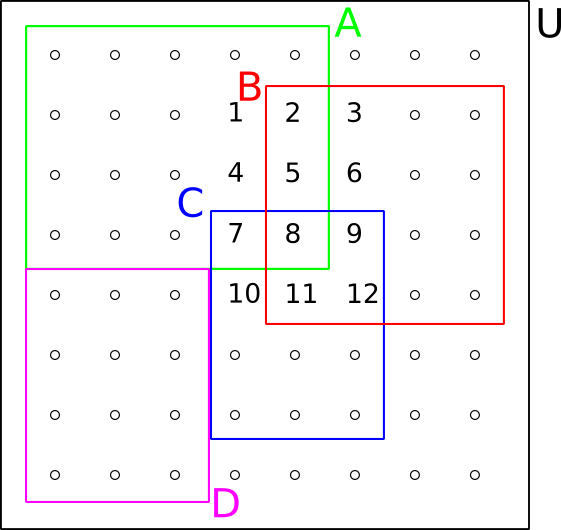
\includegraphics[width=8cm]{setcover2.png}
	\caption{Couverture par ensembles}
\end{figure}

La figure ci dessus représente un exemple de couverture par ensemble que l'on pourrait obtenir pour un ensemble donné de listes de filtres. On ne représente ici qu'un nombre limité de listes pour plus de clarté.\\

On défini $E$ l'ensemble des listes de filtres considérées, $U$ l'ensemble des règles contenues dans ces listes. On considère $A, B, C, D \in E$ et $r_1, r_2, \cdots, r_{12} \in U$. On note $\mathcal{B}$ l'ensemble des règles bloquées lors du test et $\overline{\mathcal{B}}$ l'ensemble des règles non bloquées.

Soit un test tel que :
\[ \mathcal{B} = \{r_1, r_2, r_4, r_5, r_7, r_8, r_9, r_{10}, r_{11}, r_{12}\} \]
\[ \overline{\mathcal{B}} = \{r_3, r_6\} \]

On en remarque que $A \cap B = \{r_2, r_5, r_8\} \subset \mathcal{B}$ et donc que au moins l'un de $A$ ou $B$ fait partie des listes installées. On remarque également que $\{r_3, r_6\} \subset B $ et $\{r_3, r_6\} \subset \overline{\mathcal{B}} $ et on en déduit que $B$ ne fait pas partie des listes installées.\\

On peut effectuer le même raisonnement sur les autres intersections de listes et en déduire que les listes $A$ et $C$ sont installées mais que la liste $B$ ne l'est pas.


\printbibliography

\newpage

\begin{center}
	
	\vspace{2cm}
	\renewcommand{\abstractname}{Résumé}
	\begin{abstract}
	
	Lors de ce stage blablabla

	\end{abstract}
	\textbf{Mots clés: Vie privée, }
	\vspace{\fill}	
	\renewcommand{\abstractname}{Abstract}
	\begin{abstract}
	
	During this internship blablabla

	\end{abstract}
	\textbf{Keywords: Privacy, adBlockers, }
	\vspace{2cm}

\end{center}





\end{document}